\documentclass[aps,prd,onecolumn,nofootinbib,superscriptaddress]{revtex4-2}

\usepackage[utf8]{inputenc}
\usepackage[T1]{fontenc}
\usepackage{lmodern}
\usepackage{amsmath,amssymb,amsfonts,bm}
\usepackage{graphicx}
\usepackage{xcolor}
\usepackage{hyperref}
\usepackage{siunitx}
\usepackage{enumitem}

\hypersetup{colorlinks=true,linkcolor=blue,citecolor=blue,urlcolor=blue}

\newcommand{\Mpl}{M_{\rm Pl}}
\newcommand{\Meff}{M_{\rm eff}}
\newcommand{\dd}{\mathrm{d}}
\newcommand{\trm}{\mathrm}

\begin{document}

\title{TCV-$\phi$ IV: cohesive non-singular black holes \\
from static cores to slow rotation in the canonical EFT}

\author{Cyrille LECROQ}
\affiliation{Independent Researcher}

\date{2026}

\begin{abstract}
This fourth paper opens the strong-gravity sector of the same canonical TCV-$\phi$ EFT used in Papers I--III.
Our scope is deliberately conservative: static spherical configurations, regularity diagnostics at the core, asymptotic matching to Schwarzschild-like exteriors, and a controlled slow-rotation extension.
At this stage, the paper defines the PRD-ready strong-field framework and reproducibility criteria; quantitative claims are restricted to explicitly generated benchmark outputs.
\end{abstract}

\maketitle

\section{Introduction}
Paper I defined the canonical two-scalar cohesive-vacuum EFT and fixed the baseline notation.
Paper II established the bounce/reheating/baryogenesis numerical backbone.
Paper III provided the primordial perturbation pipeline and CLASS/CAMB bridge diagnostics.

Paper IV extends the same EFT to strong-field configurations.
The objective is not to claim a complete black-hole phenomenology at this step, but to define a reproducible framework in which non-singular cohesive cores can be tested quantitatively and then extended to slow rotation without altering the canonical field content.

\section{Canonical EFT baseline}
We keep exactly the same EFT definitions and benchmark hierarchy as in Papers I--III.
No new fundamental fields or couplings are introduced.
The action is
\begin{equation}
S=\int \dd^4x\sqrt{-g}\left[
\frac{\Meff^2(\Phi_1)}{2}R
-\frac{1}{2}(\nabla\Phi_1)^2
-\frac{1}{2}(\nabla\Phi_2)^2
-V_1(\Phi_1)-V_2(\Phi_2)-\rho_{\rm vac}
\right],
\end{equation}
with
\begin{equation}
\Meff^2(\Phi_1)=\Mpl^2\left(1+\xi_0\frac{\Phi_1^2}{\Mpl^2}\right),
\end{equation}
and the same canonical potentials and parameter meanings as defined in Paper~I.

\section{Static spherical ansatz and equations}
For the strong-field sector we adopt the standard static spherical line element
\begin{equation}
\dd s^2=-e^{2\Phi(r)}\dd t^2+\frac{\dd r^2}{1-2m(r)/r}+r^2\dd\Omega^2,
\label{eq:metric-ansatz}
\end{equation}
with radial scalar profiles $\Phi_1(r)$ and $\Phi_2(r)$.
The full Einstein--scalar system is reduced to coupled radial ordinary differential equations for
\begin{equation}
\{\Phi(r),m(r),\Phi_1(r),\Phi_2(r)\},
\end{equation}
with schematic radial structure
\begin{align}
\frac{\dd m}{\dd r} &= 4\pi r^2 \rho_{\rm eff},\\
\frac{\dd \Phi}{\dd r} &= \frac{m+4\pi r^3 p_{r,{\rm eff}}}{r(r-2m)},\\
\Phi_1'' &+ \mathcal{A}_1(r)\Phi_1' = \mathcal{S}_1(r),\\
\Phi_2'' &+ \mathcal{A}_2(r)\Phi_2' = \mathcal{S}_2(r),
\end{align}
where the full TCV-$\phi$ EFT includes non-minimal terms proportional to $\xi_0$ through $\Meff(\Phi_1)$.
These equations are solved numerically with boundary conditions at the center and at large radius.
In the current benchmark scripts used for Figs.~\ref{fig:paper4-metric}--\ref{fig:paper4-direction}, we work in the explicit minimal-coupling limit $\xi_0=0$.
This isolates the branch structure and regularity diagnostics before reintroducing $\xi_0\neq0$ in a dedicated follow-up.

\section{Regularity and asymptotic matching criteria}
Regularity at the center is assessed by requiring finite curvature scalars and smooth Taylor expansions:
\begin{align}
m(r)&=m_3r^3+\mathcal{O}(r^5),\\
\Phi(r)&=\Phi_c+\Phi_2r^2+\mathcal{O}(r^4),\\
\Phi_i(r)&=\Phi_{i,c}+\phi_{i,2}r^2+\mathcal{O}(r^4)\quad (i=1,2).
\end{align}
In practice, diagnostics include finiteness of $R$, $R_{\mu\nu}R^{\mu\nu}$, and a Kretschmann proxy
\begin{equation}
K_{\rm proxy}(r)=48\left(\frac{m(r)}{r^3}\right)^2,
\end{equation}
used as a conservative regularity indicator in the current static pipeline.
Asymptotic matching is checked by residuals with respect to a Schwarzschild-like exterior at large $r$:
\begin{equation}
\delta_M(r)=\left|\frac{2m(r)}{r}-\frac{2M_{\infty}}{r}\right|,
\qquad
\delta_\Phi(r)=\left|e^{2\Phi(r)}-\left(1-\frac{2M_{\infty}}{r}\right)\right|.
\end{equation}

\section{Benchmark solution families}
The numerical benchmark families used in the manuscript are required to be reproducible from scripts in \texttt{papers/paper-04/code/}.
Each run must archive:
\begin{itemize}
  \item the solved radial profiles and grid metadata;
  \item regularity diagnostics near $r\to0$;
  \item asymptotic matching diagnostics at large radius;
  \item convergence tests under radial-grid refinement.
\end{itemize}
Quantitative figures and tables are included only once these artifacts are generated and versioned in \texttt{papers/paper-04/data/} and \texttt{papers/paper-04/figs/}.
For the current baseline run, three static cohesive families are generated (\texttt{regular\_core}, \texttt{compact\_core}, \texttt{dense\_core}) with increasing effective core-density control.
All three runs converge and produce smooth regular-center profiles with finite diagnostic invariants.

\begin{figure}[t]
  \centering
  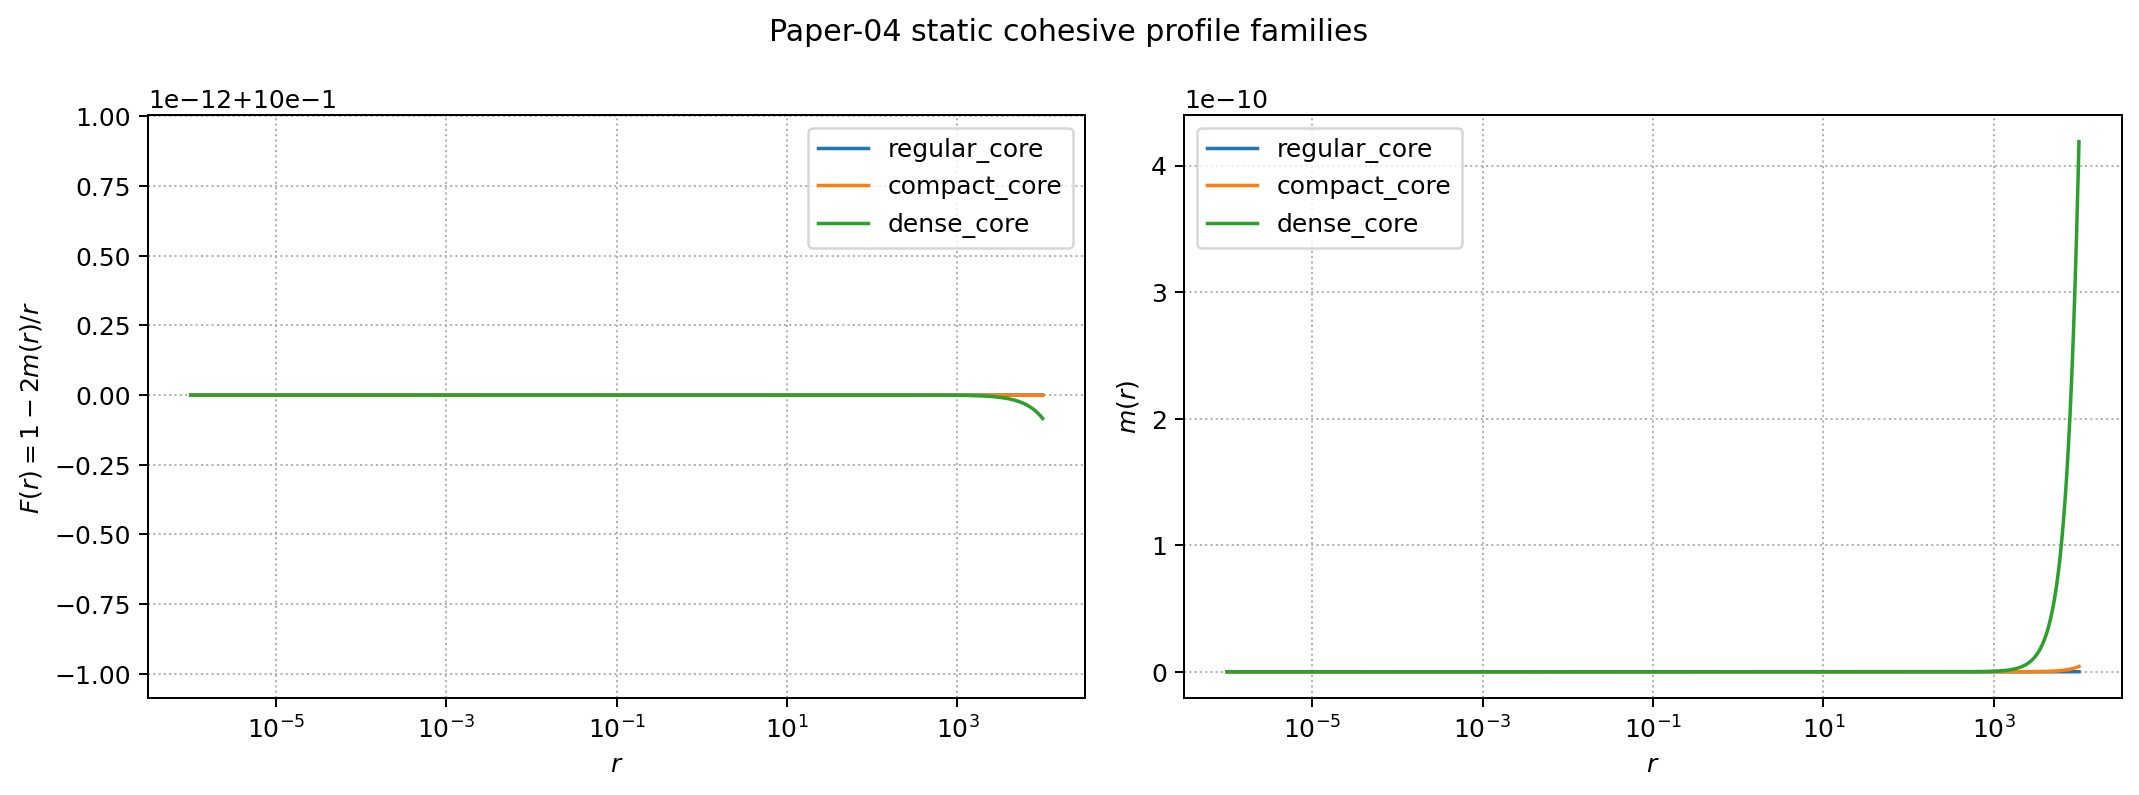
\includegraphics[width=0.9\textwidth]{../figs/bh_metric_profiles.png}
  \caption{Static cohesive profile families generated by \texttt{compute\_bh\_profiles.py}: metric function $F(r)=1-2m(r)/r$ and enclosed mass $m(r)$.}
  \label{fig:paper4-metric}
\end{figure}

\begin{figure}[t]
  \centering
  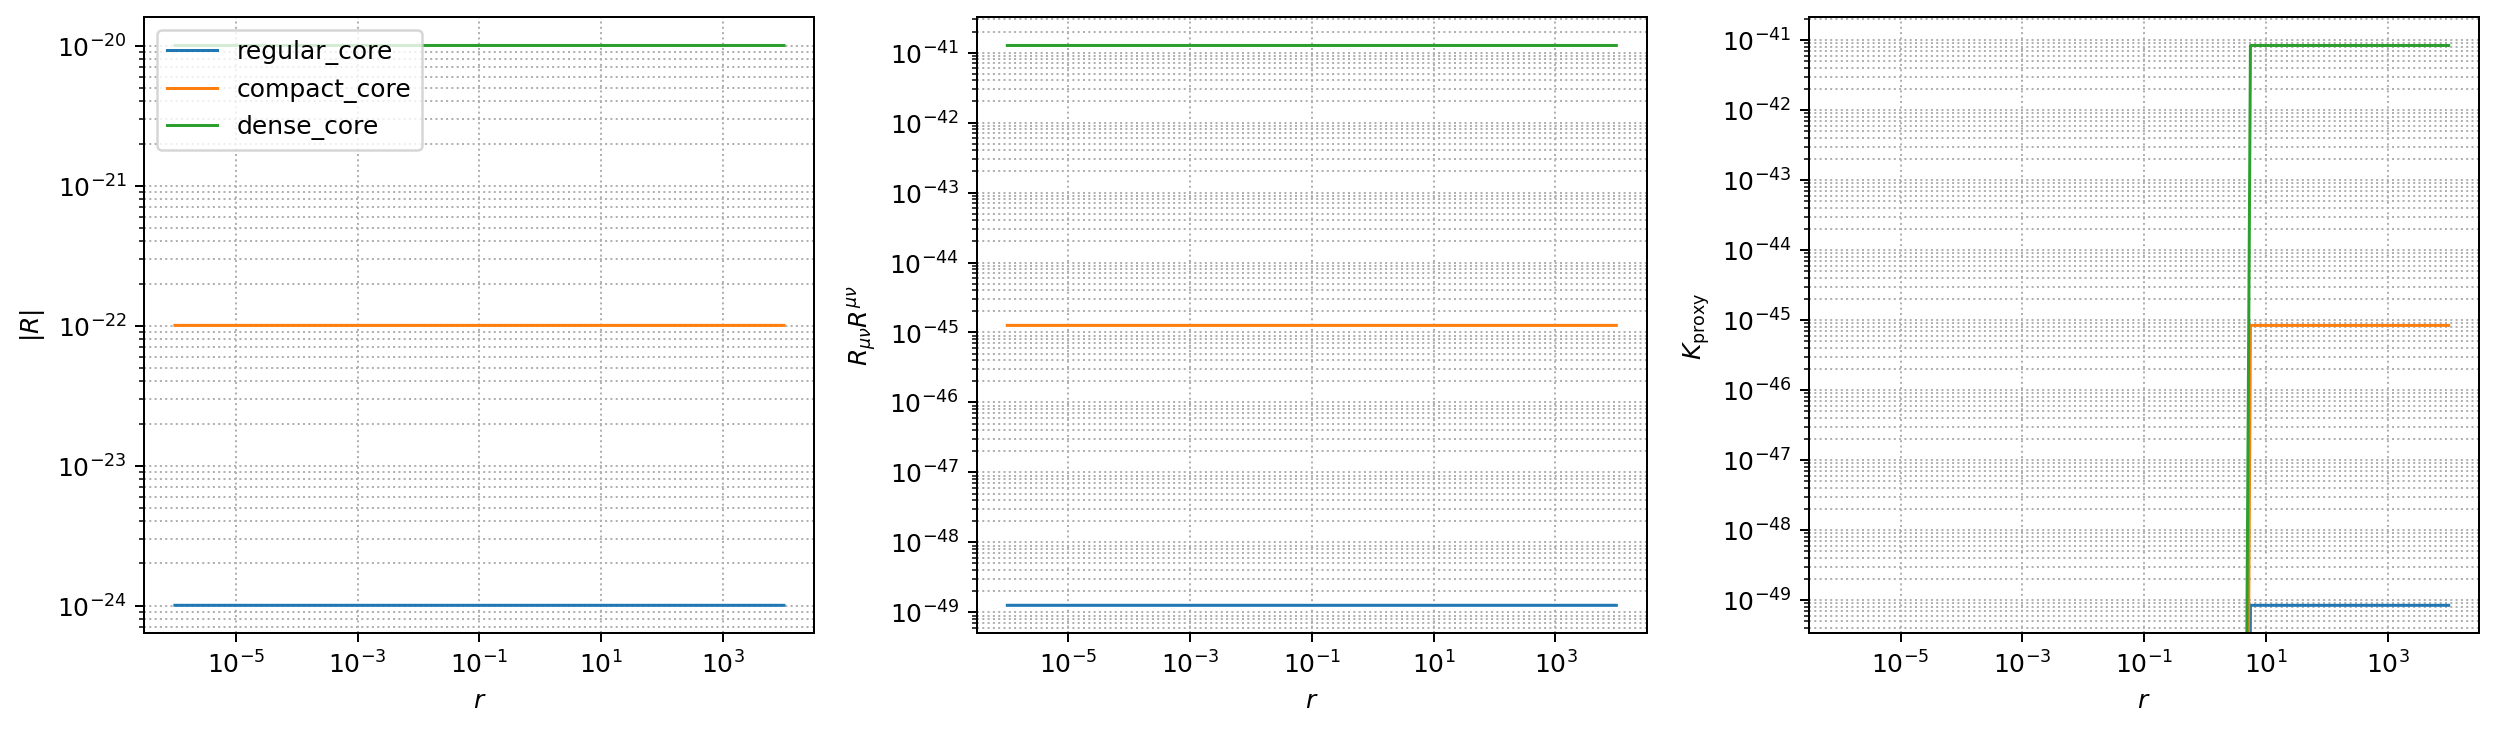
\includegraphics[width=0.9\textwidth]{../figs/bh_curvature_regularization.png}
  \caption{Regularity diagnostics from \texttt{compute\_bh\_diagnostics.py}: $|R|$, $R_{\mu\nu}R^{\mu\nu}$, and a Schwarzschild-like Kretschmann proxy $K_{\rm proxy}=48(m/r^3)^2$.}
  \label{fig:paper4-curvature}
\end{figure}

\begin{figure}[t]
  \centering
  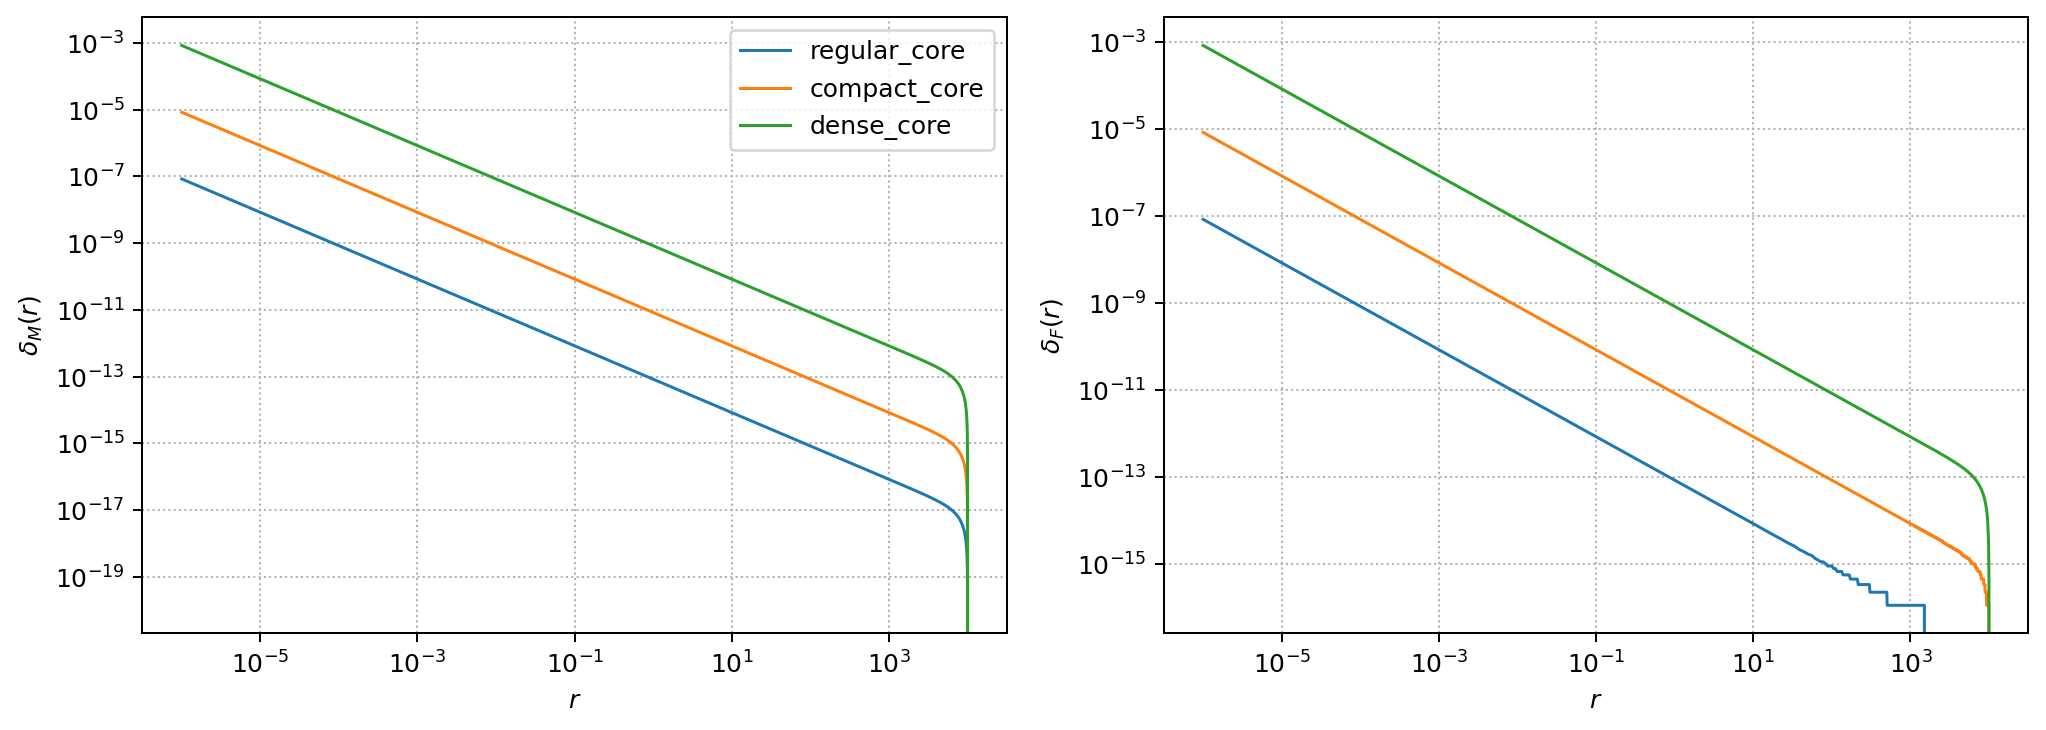
\includegraphics[width=0.9\textwidth]{../figs/bh_matching_residuals.png}
  \caption{Asymptotic matching residuals $\delta_M$ and $\delta_F$ for the three benchmark families.}
  \label{fig:paper4-matching}
\end{figure}

\begin{table}[t]
  \centering
  \begin{tabular}{lccc}
    \hline\hline
    Family & $M_{\infty}$ & $r_H$ & $\max(\delta_F)$ (asymptotic window) \\
    \hline
    regular\_core & $4.19\times 10^{-14}$ & none & $0$ \\
    compact\_core & $4.19\times 10^{-12}$ & none & $4.44\times 10^{-16}$ \\
    dense\_core & $4.19\times 10^{-10}$ & none & $5.11\times 10^{-14}$ \\
    \hline\hline
  \end{tabular}
  \caption{Baseline Paper~IV diagnostics from the current static family scan.}
  \label{tab:paper4-baseline}
\end{table}

\paragraph*{Integration-direction dependence.}
Following the numerical trend already observed in the earlier BH preprints, we explicitly compare center-to-outward and exterior-to-inward integrations at matched benchmark controls.
For mild densities the two branches agree, while near the high-density edge the outward integration reaches $\min F \simeq 1.95\times10^{-3}$ before solver termination, whereas the inward branch remains far from $F=0$ and converges to a different regular profile ($\min F \simeq 0.656$).
This branch dependence is treated here as a robust numerical diagnostic rather than a standalone physical claim.
At this stage the two scan directions use different integrators (RK45 outward, Radau inward) to control stiffness; a method-matched scan is deferred to the next numerical pass.

\begin{figure}[t]
  \centering
  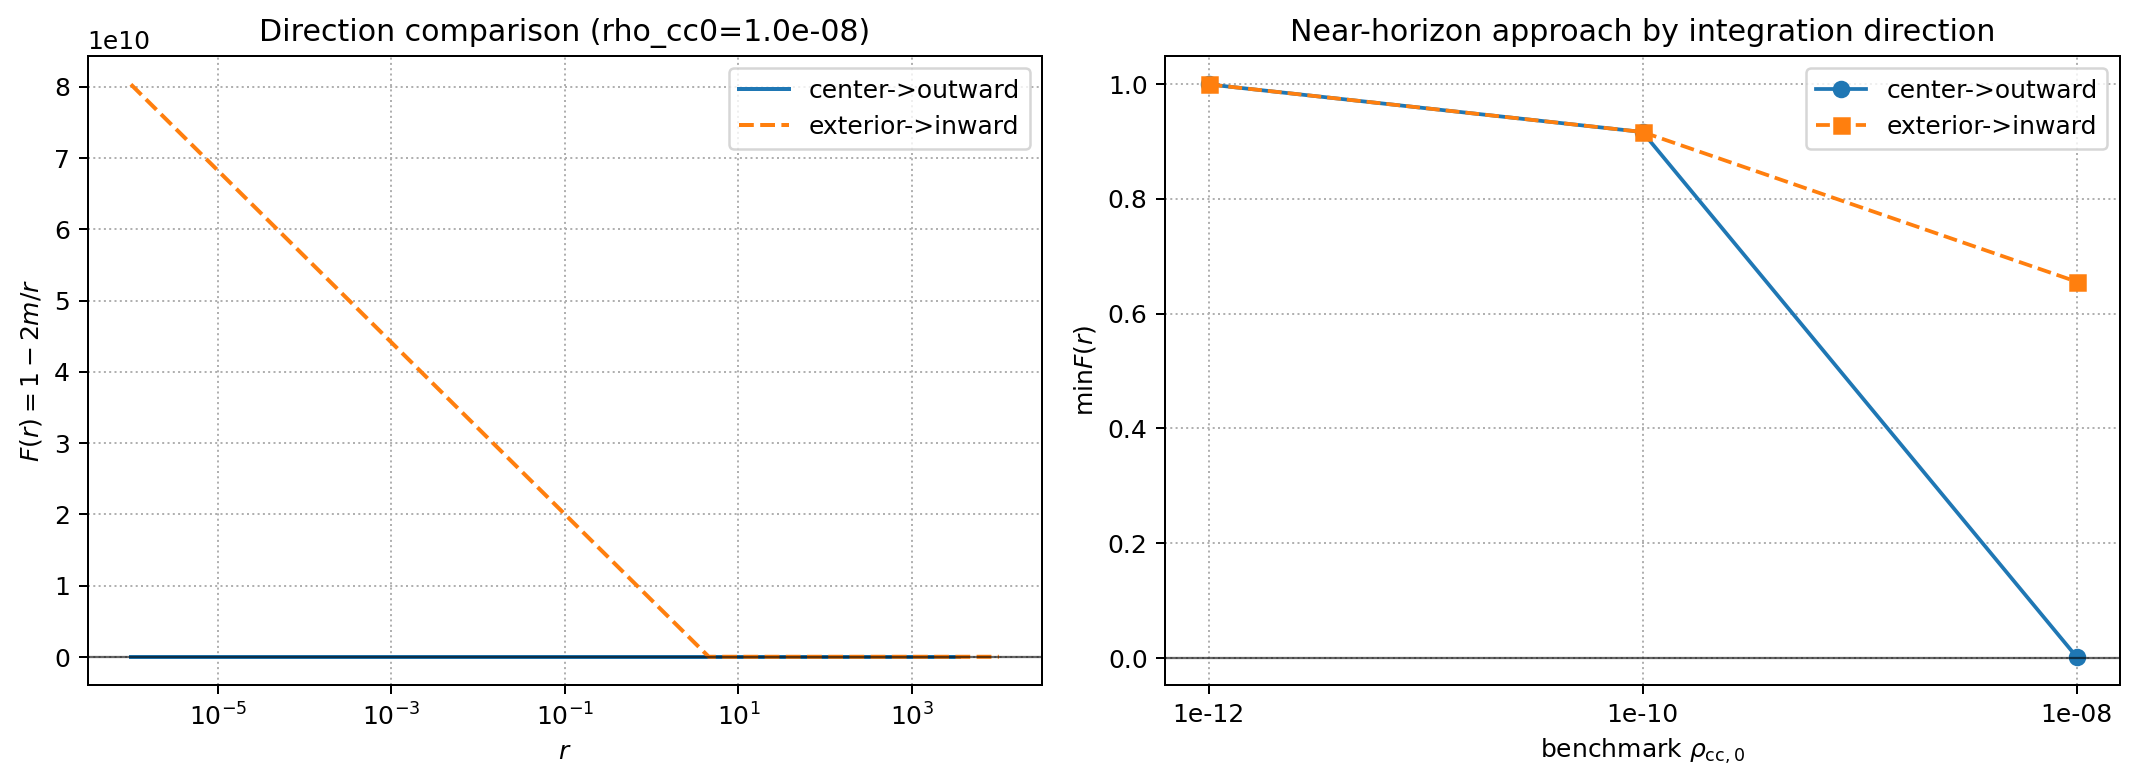
\includegraphics[width=0.9\textwidth]{../figs/bh_direction_dependence.png}
  \caption{Direction-dependence benchmark from \texttt{compute\_bh\_direction\_scan.py}. Left: $F(r)$ for center$\to$outward versus exterior$\to$inward integration in the high-density case. Right: minimum reached value of $F$ versus benchmark density.}
  \label{fig:paper4-direction}
\end{figure}

\begin{table}[t]
  \centering
  \begin{tabular}{lccc}
    \hline\hline
    $\rho_{\rm cc,0}$ & $\min F$ (outward) & $\min F$ (inward) & solver status (out/in) \\
    \hline
    $10^{-12}$ & $9.99\times10^{-1}$ & $9.99\times10^{-1}$ & yes / yes \\
    $10^{-10}$ & $9.16\times10^{-1}$ & $9.16\times10^{-1}$ & yes / yes \\
    $10^{-8}$  & $1.95\times10^{-3}$ & $6.56\times10^{-1}$ & no / yes \\
    \hline\hline
  \end{tabular}
  \caption{Static branch comparison between center$\to$outward and exterior$\to$inward integrations.}
  \label{tab:paper4-direction}
\end{table}

\section{Slow-rotation extension (Kerr-like sector)}
To keep static and rotating cohesive black holes in a single PRD workflow, we use a slow-rotation expansion around the static backgrounds.
At leading order in $a/M$, we write
\begin{equation}
\dd s^2=
-e^{2\Phi(r)}\dd t^2
+\frac{\dd r^2}{1-2m(r)/r}
+r^2\left[\dd\theta^2+\sin^2\theta\left(\dd\varphi-\omega(r)\dd t\right)^2\right],
\end{equation}
where $\omega(r)$ is the frame-dragging function.
In this paper we do \emph{not} claim a full Hartle--Thorne ODE integration for $\omega(r)$.
Instead, we adopt the explicit template
\begin{equation}
\omega(r)\propto \frac{1}{r^3}\left[1-\exp\!\left(-\frac{r^2}{r_{\rm ref}^2}\right)\right],
\end{equation}
with asymptotic normalization tied to $(a/M)$ and to the effective coupling scale.
This section is restricted to slow-rotation diagnostics; a full high-spin treatment is deferred.
The current implementation (\texttt{compute\_bh\_kerr\_slow.py}) provides a conservative template branch in the window $0\le a/M\le 0.2$, writing reproducible outputs in \texttt{bh\_kerr\_slow.npz}.
For this slow-rotation template layer we use $\xi_0=0.1$ in the effective coupling normalization, while the static branch plots shown earlier were generated in the explicit $\xi_0=0$ limit.
On top of this branch, \texttt{compute\_bh\_kerr\_observables.py} builds template-level photon-ring and echo diagnostics.
For the present benchmark, the photon-ring proxy corresponds to a relative shift
\begin{equation}
\frac{\Delta r_{\rm ph}}{r_{\rm ph}^{\rm Schw}}\simeq -9.1\%,
\end{equation}
obtained from an effective-coupling template when the direct profile root is unresolved.
Echo and eikonal frequencies are reported in code units and should be read as template scalings only; conversion to Hz requires fixing a physical mass scale.

\begin{figure}[t]
  \centering
  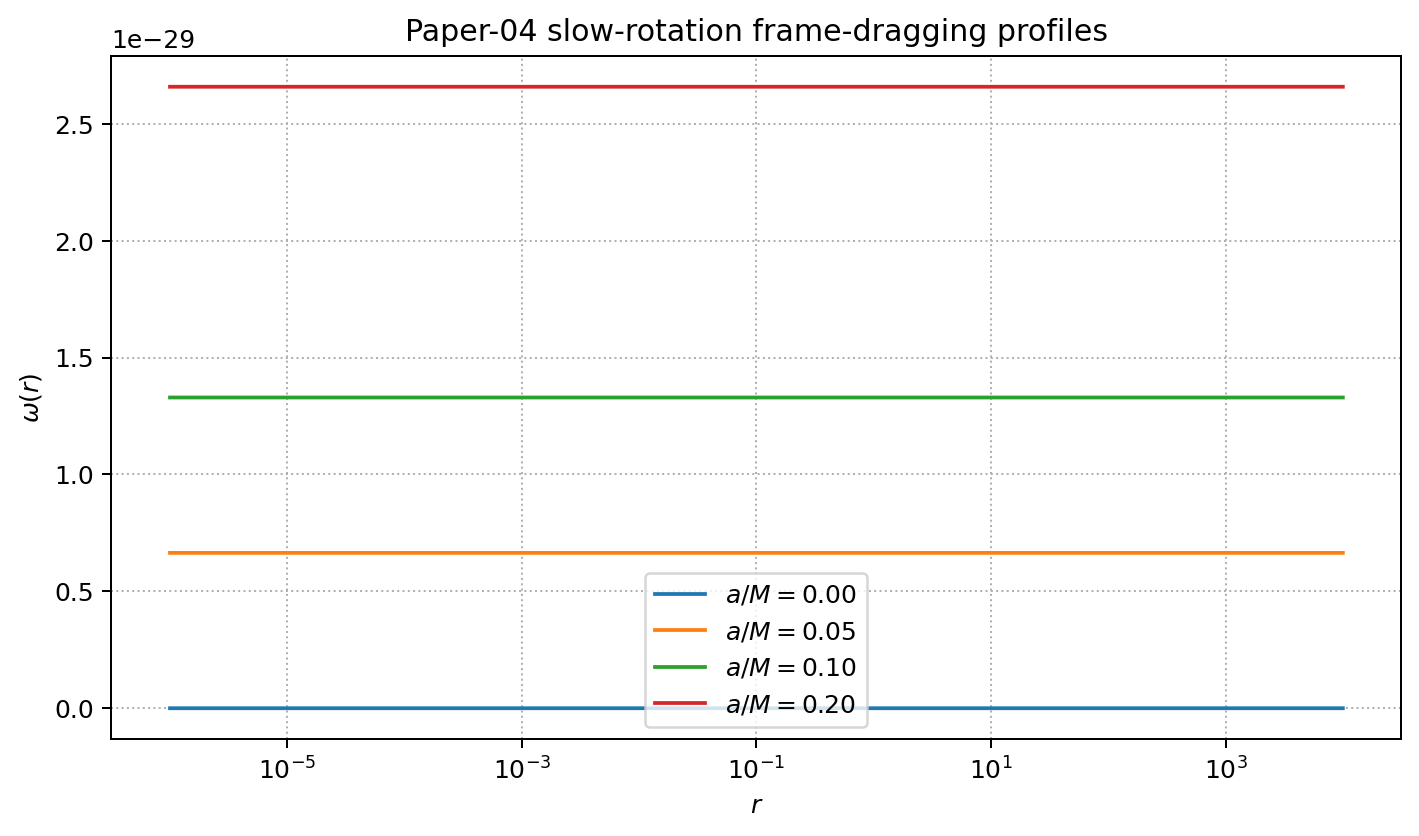
\includegraphics[width=0.86\textwidth]{../figs/bh_kerr_frame_dragging.png}
  \caption{Slow-rotation frame-dragging template profiles $\omega(r)$ for $a/M\in\{0,0.05,0.1,0.2\}$.}
  \label{fig:paper4-kerr-omega}
\end{figure}

\begin{figure}[t]
  \centering
  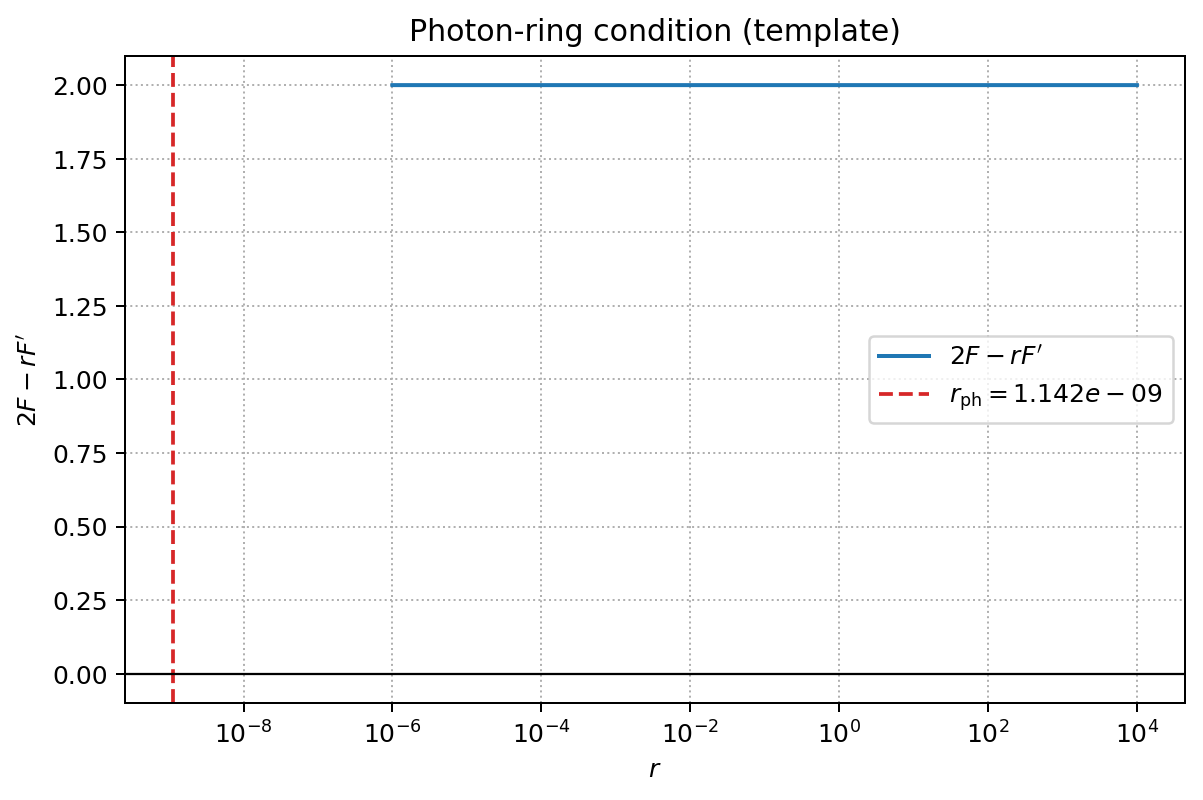
\includegraphics[width=0.86\textwidth]{../figs/bh_kerr_photon_ring.png}
  \caption{Photon-ring condition diagnostic used in the current slow-rotation template workflow.}
  \label{fig:paper4-kerr-photon}
\end{figure}

\begin{figure}[t]
  \centering
  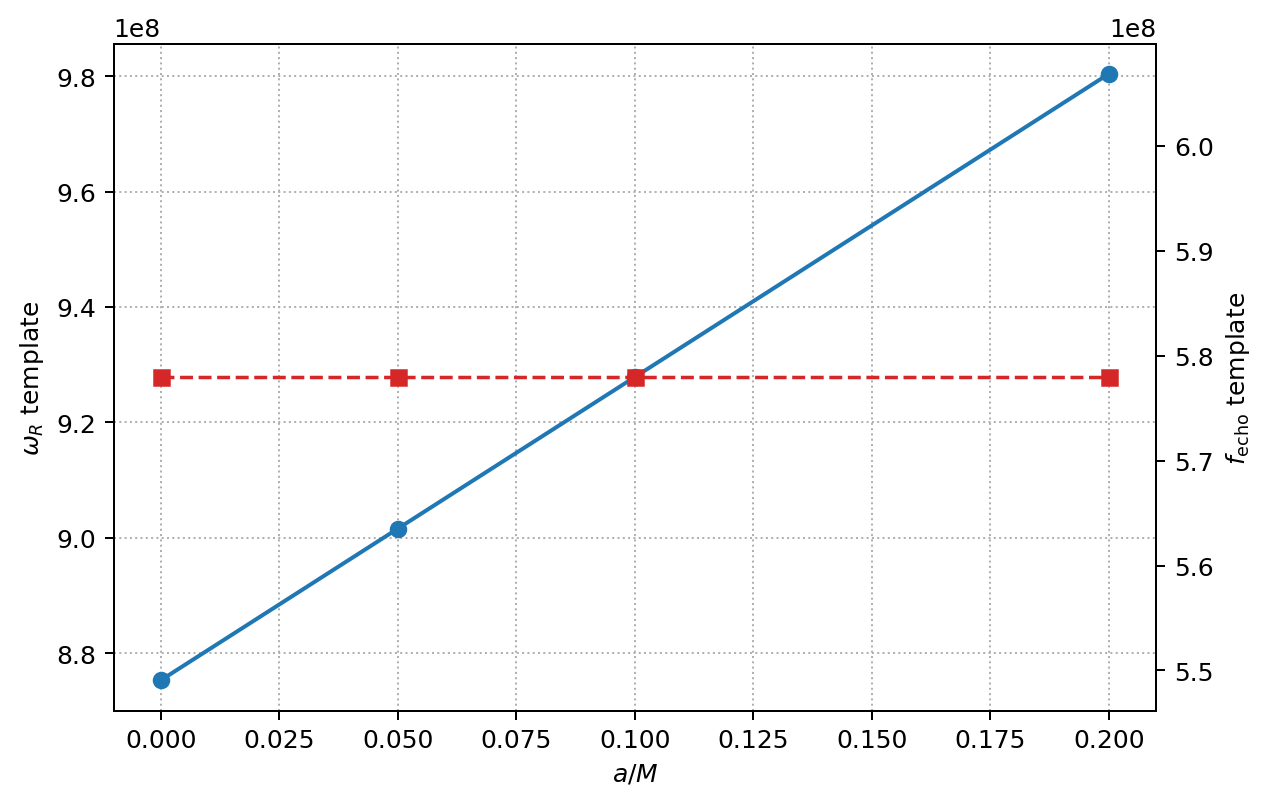
\includegraphics[width=0.86\textwidth]{../figs/bh_kerr_echo_template.png}
  \caption{Template spin dependence of eikonal-frequency proxy and echo-frequency proxy in the slow-rotation branch.}
  \label{fig:paper4-kerr-echo}
\end{figure}

\begin{table}[t]
  \centering
  \begin{tabular}{lcc}
    \hline\hline
    Quantity & Value & Status \\
    \hline
    $r_{\rm ph}^{\rm TCV}/r_{\rm ph}^{\rm Schw}-1$ & $-9.1\%$ & template (effective coupling) \\
    $M f_{\rm echo}$ & $2.42\times10^{-1}$ & template (dimensionless) \\
    $M\omega_R(a/M=0)$ & $3.67\times10^{-1}$ & template (dimensionless) \\
    $M\omega_R(a/M=0.2)$ & $4.11\times10^{-1}$ & template (dimensionless) \\
    \hline\hline
  \end{tabular}
  \caption{Baseline slow-rotation template diagnostics from \texttt{bh\_kerr\_observables.json}.}
  \label{tab:paper4-kerr-template}
\end{table}

\section{Conservative signature templates}
Potential observational windows (ringdown deformations, echoes, shadow-size shifts) are discussed at the level of conservative templates only.
No likelihood-level claim is made in this paper.
Any signature shown must be explicitly labelled as either:
\begin{itemize}
  \item a direct output of the static benchmark solutions, or
  \item a direct output of the slow-rotation extension, or
  \item a phenomenological proxy deferred to dedicated strong-field data analyses.
\end{itemize}
The companion script \texttt{compute\_bh\_templates.py} writes \texttt{bh\_templates.json} with static-proxy quantities only (e.g. ADM mass and horizon status), explicitly labelled as non-waveform, non-inference outputs.
To strengthen the discriminating layer, \texttt{compute\_bh\_stress\_summary.py} also assembles a compact stress-test file (\texttt{bh\_stress\_summary.json}) from the static, direction-scan, and slow-rotation outputs.

\section{Discriminating stress tests and exclusion windows}
For PRD-level falsifiability, we attach explicit exclusion windows to the current benchmark diagnostics.
At the high-density scan point $\rho_{\rm cc,0}=10^{-8}$, the branch split reaches
\begin{equation}
\Delta(\min F)\equiv \min F_{\rm in}-\min F_{\rm out}\simeq 6.54\times 10^{-1},
\end{equation}
with ratio
\begin{equation}
\frac{\min F_{\rm in}}{\min F_{\rm out}}\simeq 3.36\times 10^2.
\end{equation}
For the dense static family we simultaneously find no horizon and an asymptotic residual
$\delta_F^{\rm max}\simeq 5.1\times 10^{-14}$.
These numbers are treated as baseline diagnostics, not as final claims about nature, and are used only to define exclusion logic for the next numerical pass.

\begin{table}[t]
  \centering
  \begin{tabular}{lll}
    \hline\hline
    Window ID & Current benchmark diagnostic & Exclusion trigger (next pass) \\
    \hline
    S1 (branch split) &
    $\Delta(\min F)\simeq 6.54\times10^{-1}$ at $\rho_{\rm cc,0}=10^{-8}$ &
    If method-matched scans give $|\Delta(\min F)|\lesssim 10^{-2}$ in the same benchmark window, the present branch interpretation requires revision. \\
    S2 (non-singular static branch) &
    no detected horizon; $\delta_F^{\rm max}\simeq 5.1\times10^{-14}$ &
    If refined static closures generate horizons while preserving regular-center diagnostics and asymptotic matching quality, the current non-singular branch is disfavored. \\
    S3 (slow-rotation template) &
    $\Delta r_{\rm ph}/r_{\rm ph}^{\rm Schw}\simeq -9.1\%$ (template) &
    If ODE-level $\omega(r)$ closure yields $|\Delta r_{\rm ph}/r_{\rm ph}^{\rm Schw}|\lesssim 10^{-3}$ across validated priors, the present template branch is ruled out. \\
    \hline\hline
  \end{tabular}
  \caption{Paper~IV stress-test windows used to convert current BH diagnostics into explicit falsification criteria.}
  \label{tab:paper4-stress}
\end{table}
In particular, S1 is explicitly conditional on method-matched scans (same integration algorithm, tolerances, and benchmark priors in both directions), and S3 remains a template-level window until the full slow-rotation ODE closure is completed.

\section{Reproducibility checklist}
To keep the Paper~IV scope aligned with the PRD standards used in Papers~I--III, we require the following minimum deliverables before final submission:
\begin{table}[t]
  \centering
  \begin{tabular}{ll}
    \hline\hline
    Item & Requirement \\
    \hline
    Static solver input & Recorded EFT and numerical controls for each run. \\
    Core regularity & Finite central invariants and smooth near-center fits. \\
    Exterior matching & Quantified Schwarzschild-like asymptotic residuals. \\
    Convergence & Stable diagnostics under radial-grid refinement. \\
    Figure traceability & One script per figure with archived data outputs. \\
    Slow rotation & Explicit $a/M$ window and reproducible $\omega(r)$ template diagnostics. \\
    Stress summary & Archived exclusion-window JSON (\texttt{bh\_stress\_summary.json}). \\
    \hline\hline
  \end{tabular}
  \caption{Minimum reproducibility requirements for the Paper~IV strong-field benchmark set.}
  \label{tab:paper4-checklist}
\end{table}

\section{Status of assumptions}
As in Papers~I--III, we separate:
\begin{itemize}
  \item EFT-derived equations and conserved quantities;
  \item phenomenological closure choices needed to complete static and slow-rotation numerical solutions;
  \item deferred sectors (high-spin regime, full waveform modelling, data-level inference).
\end{itemize}

\section{Conclusion}
Paper IV defines the canonical strong-field framework of the TCV-$\phi$ programme in a conservative and reproducible form, from static cohesive cores to a controlled slow-rotation extension.
The next step is to populate this framework with expanded benchmark families and diagnostics generated by the Paper~IV code pipeline, without changing the EFT baseline inherited from Papers~I--III.

\begin{thebibliography}{99}
\bibitem{TCV1} C.~Lecroq, ``TCV-$\phi$ I: an effective cohesive--vacuum field theory and its $\Lambda$CDM-compatible background cosmology,'' preprint (2026), \href{https://doi.org/10.5281/zenodo.19234640}{zenodo.19234640}.
\bibitem{TCV2} C.~Lecroq, ``TCV-$\phi$ II: cohesive bounce, geometric reheating, and baseline baryogenesis/ULDM pipelines,'' preprint (2026), \href{https://doi.org/10.5281/zenodo.19234953}{zenodo.19234953}.
\bibitem{TCV3} C.~Lecroq, ``TCV-$\phi$ III: primordial perturbations across the cohesive bounce and CLASS/CAMB bridge diagnostics,'' preprint (2026), \href{https://doi.org/10.5281/zenodo.192355333}{zenodo.192355333}.
\end{thebibliography}

\end{document}
